\documentclass[a4paper, 12pt]{article}
\usepackage[left = 13 mm, top = 15mm, right = 13 mm, bottom = 23mm, bindingoffset = 7mm]{geometry}
\usepackage[T2A,T1]{fontenc}
\usepackage[utf8]{inputenc}
\usepackage[english,russian]{babel}
\usepackage{graphicx}
\usepackage{amssymb, mathtools}
\usepackage{lipsum}
\usepackage{float}
\usepackage{wrapfig}
\usepackage{indentfirst} 

\newcommand{\HRule}{\rule{\linewidth}{0.3mm}}

\newcommand{\LabTitle}{Исследование сдвига фаз в RLC-цепях}
\begin{document}




\begin{titlepage}
\begin{center}\large
ФГАУ ВПО <<МОСКОВСКИЙ ФИЗИКО-ТЕХНИЧЕСКИЙ УНИВЕРСИТЕТ>>
\begin{figure}[H]
\centering

\includegraphics[width=15cm]{logo.jpg}
\end{figure}
{\Large
Кафедра радиотехники}

\vfill

\hrule
\vspace{0.3cm}

\huge \LabTitle

\vspace{0.3cm}
\hrule


%\noindent\rule{\textwidth}{0.4mm}
%\huge Магнитометр
%\noindent\rule{\textwidth}{0.4mm}


\end{center}

\vfill


\begin{minipage}{0.7\textwidth}
\textbf{Выполнил:}
Корепанов Г.М.

512 группа

\vspace{0.5cm}

\textbf{Преподаватель:}
Филатов Иван Васильевич
\end{minipage}


\vfill
\centering
 Долгопрудный, 2016 г.




\end{titlepage}


\section*{Экспериментальная установка}
\begin {figure}[H]
\begin{center}
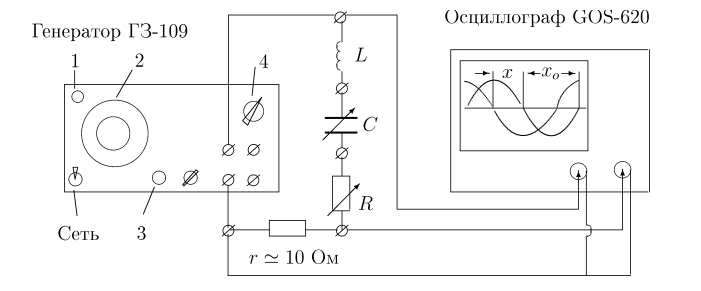
\includegraphics[width=0.9\textwidth]{t}
\end{center}
\end {figure}
$$R_L=45,6 \text{ Ом}$$
$$L=50 \text{ мГн}$$
$$r=10 \text { Ом}$$
$$C=0,5 \text{ мкФ}$$
\section*{RC-цепочка, теория}
Ток, текущий через RC цепочку, пропорционален напряжению на резисторе, и опережает напряжение на конденсаторе по фазе на $\pi/2$. В таком простом случае метод векторных диаграмм даёт простой результат для зависимости сдвига фаз от $R$:
$$\tg\varphi = \frac{1}{\omega R C}$$
\begin {figure}[H]
\begin{center}
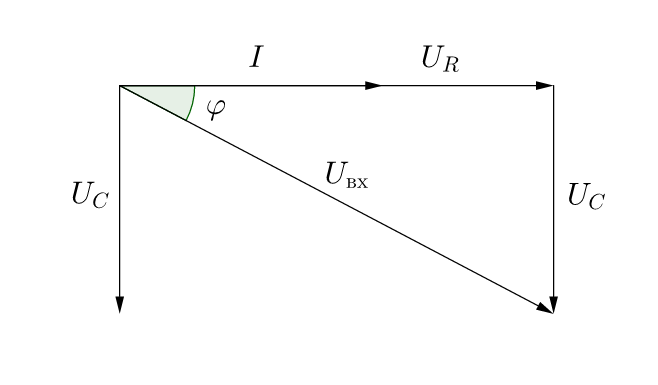
\includegraphics[width=0.7\textwidth]{rcd}
\end{center}
\end {figure}

\section*{RC-цепочка, эксперимент}
\begin {figure}[H]
\begin{center}
\scalebox{.95}{% GNUPLOT: LaTeX picture with Postscript
\begingroup
  \fontfamily{sansserif}%
  \selectfont
  \makeatletter
  \providecommand\color[2][]{%
    \GenericError{(gnuplot) \space\space\space\@spaces}{%
      Package color not loaded in conjunction with
      terminal option `colourtext'%
    }{See the gnuplot documentation for explanation.%
    }{Either use 'blacktext' in gnuplot or load the package
      color.sty in LaTeX.}%
    \renewcommand\color[2][]{}%
  }%
  \providecommand\includegraphics[2][]{%
    \GenericError{(gnuplot) \space\space\space\@spaces}{%
      Package graphicx or graphics not loaded%
    }{See the gnuplot documentation for explanation.%
    }{The gnuplot epslatex terminal needs graphicx.sty or graphics.sty.}%
    \renewcommand\includegraphics[2][]{}%
  }%
  \providecommand\rotatebox[2]{#2}%
  \@ifundefined{ifGPcolor}{%
    \newif\ifGPcolor
    \GPcolorfalse
  }{}%
  \@ifundefined{ifGPblacktext}{%
    \newif\ifGPblacktext
    \GPblacktexttrue
  }{}%
  % define a \g@addto@macro without @ in the name:
  \let\gplgaddtomacro\g@addto@macro
  % define empty templates for all commands taking text:
  \gdef\gplbacktext{}%
  \gdef\gplfronttext{}%
  \makeatother
  \ifGPblacktext
    % no textcolor at all
    \def\colorrgb#1{}%
    \def\colorgray#1{}%
  \else
    % gray or color?
    \ifGPcolor
      \def\colorrgb#1{\color[rgb]{#1}}%
      \def\colorgray#1{\color[gray]{#1}}%
      \expandafter\def\csname LTw\endcsname{\color{white}}%
      \expandafter\def\csname LTb\endcsname{\color{black}}%
      \expandafter\def\csname LTa\endcsname{\color{black}}%
      \expandafter\def\csname LT0\endcsname{\color[rgb]{1,0,0}}%
      \expandafter\def\csname LT1\endcsname{\color[rgb]{0,1,0}}%
      \expandafter\def\csname LT2\endcsname{\color[rgb]{0,0,1}}%
      \expandafter\def\csname LT3\endcsname{\color[rgb]{1,0,1}}%
      \expandafter\def\csname LT4\endcsname{\color[rgb]{0,1,1}}%
      \expandafter\def\csname LT5\endcsname{\color[rgb]{1,1,0}}%
      \expandafter\def\csname LT6\endcsname{\color[rgb]{0,0,0}}%
      \expandafter\def\csname LT7\endcsname{\color[rgb]{1,0.3,0}}%
      \expandafter\def\csname LT8\endcsname{\color[rgb]{0.5,0.5,0.5}}%
    \else
      % gray
      \def\colorrgb#1{\color{black}}%
      \def\colorgray#1{\color[gray]{#1}}%
      \expandafter\def\csname LTw\endcsname{\color{white}}%
      \expandafter\def\csname LTb\endcsname{\color{black}}%
      \expandafter\def\csname LTa\endcsname{\color{black}}%
      \expandafter\def\csname LT0\endcsname{\color{black}}%
      \expandafter\def\csname LT1\endcsname{\color{black}}%
      \expandafter\def\csname LT2\endcsname{\color{black}}%
      \expandafter\def\csname LT3\endcsname{\color{black}}%
      \expandafter\def\csname LT4\endcsname{\color{black}}%
      \expandafter\def\csname LT5\endcsname{\color{black}}%
      \expandafter\def\csname LT6\endcsname{\color{black}}%
      \expandafter\def\csname LT7\endcsname{\color{black}}%
      \expandafter\def\csname LT8\endcsname{\color{black}}%
    \fi
  \fi
    \setlength{\unitlength}{0.0500bp}%
    \ifx\gptboxheight\undefined%
      \newlength{\gptboxheight}%
      \newlength{\gptboxwidth}%
      \newsavebox{\gptboxtext}%
    \fi%
    \setlength{\fboxrule}{0.5pt}%
    \setlength{\fboxsep}{1pt}%
\begin{picture}(9354.00,6802.00)%
    \gplgaddtomacro\gplbacktext{%
      \csname LTb\endcsname%
      \put(660,1408){\makebox(0,0)[r]{\strut{}$0$}}%
      \csname LTb\endcsname%
      \put(660,2381){\makebox(0,0)[r]{\strut{}$100$}}%
      \csname LTb\endcsname%
      \put(660,3354){\makebox(0,0)[r]{\strut{}$200$}}%
      \csname LTb\endcsname%
      \put(660,4327){\makebox(0,0)[r]{\strut{}$300$}}%
      \csname LTb\endcsname%
      \put(660,5300){\makebox(0,0)[r]{\strut{}$400$}}%
      \csname LTb\endcsname%
      \put(660,6273){\makebox(0,0)[r]{\strut{}$500$}}%
      \csname LTb\endcsname%
      \put(924,968){\makebox(0,0){\strut{}$0$}}%
      \csname LTb\endcsname%
      \put(2604,968){\makebox(0,0){\strut{}$50$}}%
      \csname LTb\endcsname%
      \put(4285,968){\makebox(0,0){\strut{}$100$}}%
      \csname LTb\endcsname%
      \put(5965,968){\makebox(0,0){\strut{}$150$}}%
      \csname LTb\endcsname%
      \put(7646,968){\makebox(0,0){\strut{}$200$}}%
      \csname LTb\endcsname%
      \put(9326,968){\makebox(0,0){\strut{}$250$}}%
      \put(1764,5787){\makebox(0,0)[l]{\strut{}$K = \left(1.927\pm0.02\right)$ нА/мм}}%
    }%
    \gplgaddtomacro\gplfronttext{%
      \csname LTb\endcsname%
      \put(-9,3840){\rotatebox{-270}{\makebox(0,0){\strut{}$I$, нА}}}%
      \put(5125,308){\makebox(0,0){\strut{}$x$, мм}}%
    }%
    \gplbacktext
    \put(0,0){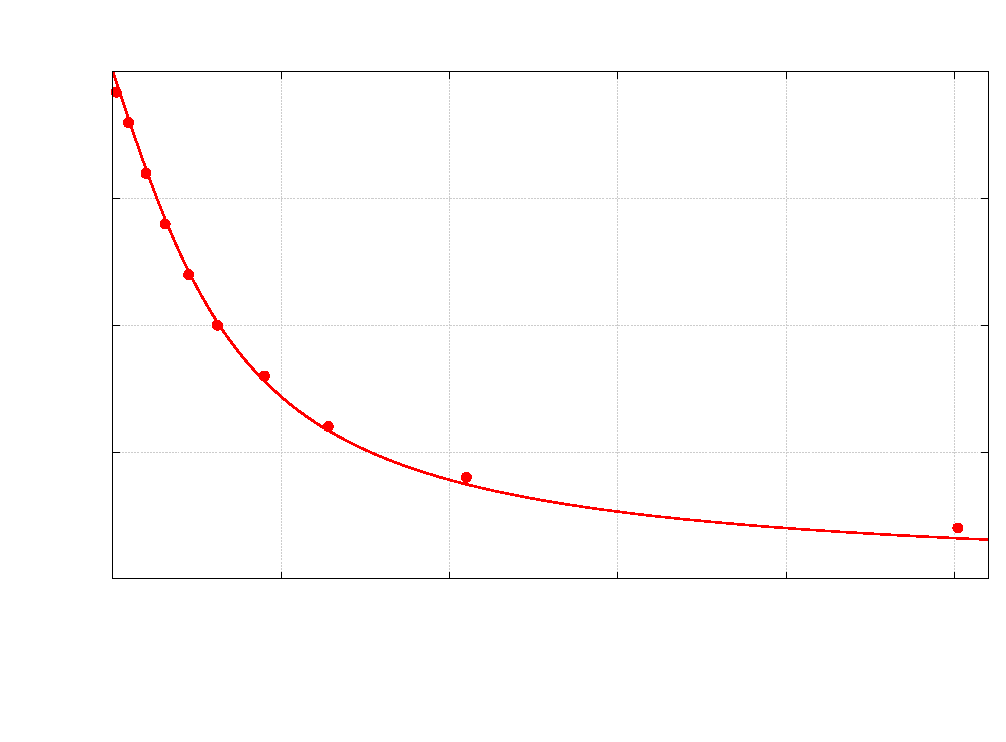
\includegraphics{plot1}}%
    \gplfronttext
  \end{picture}%
\endgroup
}
\end{center}
\end {figure}
\begin {figure}[H]
\begin{center}
\scalebox{.95}{% GNUPLOT: LaTeX picture with Postscript
\begingroup
  \fontfamily{sansserif}%
  \selectfont
  \makeatletter
  \providecommand\color[2][]{%
    \GenericError{(gnuplot) \space\space\space\@spaces}{%
      Package color not loaded in conjunction with
      terminal option `colourtext'%
    }{See the gnuplot documentation for explanation.%
    }{Either use 'blacktext' in gnuplot or load the package
      color.sty in LaTeX.}%
    \renewcommand\color[2][]{}%
  }%
  \providecommand\includegraphics[2][]{%
    \GenericError{(gnuplot) \space\space\space\@spaces}{%
      Package graphicx or graphics not loaded%
    }{See the gnuplot documentation for explanation.%
    }{The gnuplot epslatex terminal needs graphicx.sty or graphics.sty.}%
    \renewcommand\includegraphics[2][]{}%
  }%
  \providecommand\rotatebox[2]{#2}%
  \@ifundefined{ifGPcolor}{%
    \newif\ifGPcolor
    \GPcolorfalse
  }{}%
  \@ifundefined{ifGPblacktext}{%
    \newif\ifGPblacktext
    \GPblacktexttrue
  }{}%
  % define a \g@addto@macro without @ in the name:
  \let\gplgaddtomacro\g@addto@macro
  % define empty templates for all commands taking text:
  \gdef\gplbacktext{}%
  \gdef\gplfronttext{}%
  \makeatother
  \ifGPblacktext
    % no textcolor at all
    \def\colorrgb#1{}%
    \def\colorgray#1{}%
  \else
    % gray or color?
    \ifGPcolor
      \def\colorrgb#1{\color[rgb]{#1}}%
      \def\colorgray#1{\color[gray]{#1}}%
      \expandafter\def\csname LTw\endcsname{\color{white}}%
      \expandafter\def\csname LTb\endcsname{\color{black}}%
      \expandafter\def\csname LTa\endcsname{\color{black}}%
      \expandafter\def\csname LT0\endcsname{\color[rgb]{1,0,0}}%
      \expandafter\def\csname LT1\endcsname{\color[rgb]{0,1,0}}%
      \expandafter\def\csname LT2\endcsname{\color[rgb]{0,0,1}}%
      \expandafter\def\csname LT3\endcsname{\color[rgb]{1,0,1}}%
      \expandafter\def\csname LT4\endcsname{\color[rgb]{0,1,1}}%
      \expandafter\def\csname LT5\endcsname{\color[rgb]{1,1,0}}%
      \expandafter\def\csname LT6\endcsname{\color[rgb]{0,0,0}}%
      \expandafter\def\csname LT7\endcsname{\color[rgb]{1,0.3,0}}%
      \expandafter\def\csname LT8\endcsname{\color[rgb]{0.5,0.5,0.5}}%
    \else
      % gray
      \def\colorrgb#1{\color{black}}%
      \def\colorgray#1{\color[gray]{#1}}%
      \expandafter\def\csname LTw\endcsname{\color{white}}%
      \expandafter\def\csname LTb\endcsname{\color{black}}%
      \expandafter\def\csname LTa\endcsname{\color{black}}%
      \expandafter\def\csname LT0\endcsname{\color{black}}%
      \expandafter\def\csname LT1\endcsname{\color{black}}%
      \expandafter\def\csname LT2\endcsname{\color{black}}%
      \expandafter\def\csname LT3\endcsname{\color{black}}%
      \expandafter\def\csname LT4\endcsname{\color{black}}%
      \expandafter\def\csname LT5\endcsname{\color{black}}%
      \expandafter\def\csname LT6\endcsname{\color{black}}%
      \expandafter\def\csname LT7\endcsname{\color{black}}%
      \expandafter\def\csname LT8\endcsname{\color{black}}%
    \fi
  \fi
    \setlength{\unitlength}{0.0500bp}%
    \ifx\gptboxheight\undefined%
      \newlength{\gptboxheight}%
      \newlength{\gptboxwidth}%
      \newsavebox{\gptboxtext}%
    \fi%
    \setlength{\fboxrule}{0.5pt}%
    \setlength{\fboxsep}{1pt}%
\begin{picture}(9354.00,6802.00)%
    \gplgaddtomacro\gplbacktext{%
      \csname LTb\endcsname%
      \put(660,1408){\makebox(0,0)[r]{\strut{}$0$}}%
      \csname LTb\endcsname%
      \put(660,2103){\makebox(0,0)[r]{\strut{}$1$}}%
      \csname LTb\endcsname%
      \put(660,2798){\makebox(0,0)[r]{\strut{}$2$}}%
      \csname LTb\endcsname%
      \put(660,3493){\makebox(0,0)[r]{\strut{}$3$}}%
      \csname LTb\endcsname%
      \put(660,4188){\makebox(0,0)[r]{\strut{}$4$}}%
      \csname LTb\endcsname%
      \put(660,4883){\makebox(0,0)[r]{\strut{}$5$}}%
      \csname LTb\endcsname%
      \put(660,5578){\makebox(0,0)[r]{\strut{}$6$}}%
      \csname LTb\endcsname%
      \put(660,6273){\makebox(0,0)[r]{\strut{}$7$}}%
      \csname LTb\endcsname%
      \put(924,968){\makebox(0,0){\strut{}$0$}}%
      \csname LTb\endcsname%
      \put(2324,968){\makebox(0,0){\strut{}$1$}}%
      \csname LTb\endcsname%
      \put(3725,968){\makebox(0,0){\strut{}$2$}}%
      \csname LTb\endcsname%
      \put(5125,968){\makebox(0,0){\strut{}$3$}}%
      \csname LTb\endcsname%
      \put(6525,968){\makebox(0,0){\strut{}$4$}}%
      \csname LTb\endcsname%
      \put(7926,968){\makebox(0,0){\strut{}$5$}}%
      \csname LTb\endcsname%
      \put(9326,968){\makebox(0,0){\strut{}$6$}}%
    }%
    \gplgaddtomacro\gplfronttext{%
      \csname LTb\endcsname%
      \put(176,3840){\rotatebox{-270}{\makebox(0,0){\strut{}$\tg\varphi$}}}%
      \put(5125,308){\makebox(0,0){\strut{}$1/\omega R_{\sum} C$}}%
    }%
    \gplbacktext
    \put(0,0){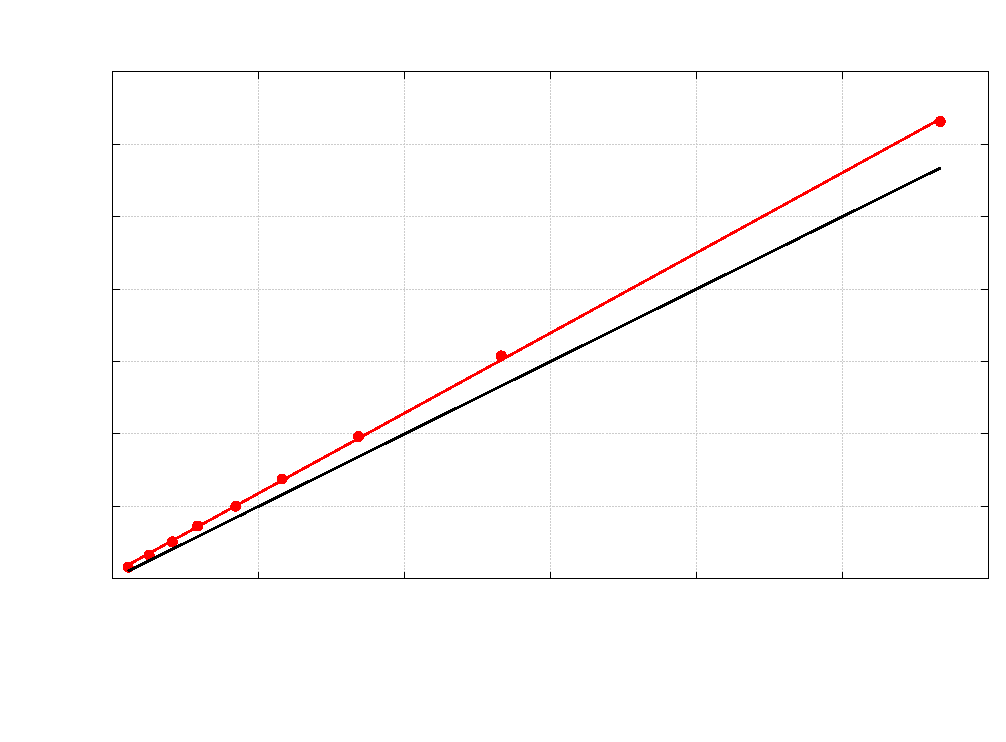
\includegraphics{plot2}}%
    \gplfronttext
  \end{picture}%
\endgroup
}
\end{center}
\end {figure}


\section*{RL-цепочка, теория}
Всё аналогично RC цепочке, только импеданс катушки теперь 
$$Z_2 = j\omega L,$$
поэтому ток отстаёт по фазе от напряжения, а рассчётная формула приобретает вид
$$\tg\varphi = \frac{\omega L}{R_{\sum}}$$
Теперь к споротивлению калибровочного резистора и резистора $R$ добавится активное сопротивление катушки:
$$R_{\sum} = R+r+R_L,$$
где $R_L$ -- активное сопротивление катушки.

\section*{RL-цепочка, эксперимент}
\begin {figure}[H]
\begin{center}
{% GNUPLOT: LaTeX picture with Postscript
\begingroup
  \fontfamily{sansserif}%
  \selectfont
  \makeatletter
  \providecommand\color[2][]{%
    \GenericError{(gnuplot) \space\space\space\@spaces}{%
      Package color not loaded in conjunction with
      terminal option `colourtext'%
    }{See the gnuplot documentation for explanation.%
    }{Either use 'blacktext' in gnuplot or load the package
      color.sty in LaTeX.}%
    \renewcommand\color[2][]{}%
  }%
  \providecommand\includegraphics[2][]{%
    \GenericError{(gnuplot) \space\space\space\@spaces}{%
      Package graphicx or graphics not loaded%
    }{See the gnuplot documentation for explanation.%
    }{The gnuplot epslatex terminal needs graphicx.sty or graphics.sty.}%
    \renewcommand\includegraphics[2][]{}%
  }%
  \providecommand\rotatebox[2]{#2}%
  \@ifundefined{ifGPcolor}{%
    \newif\ifGPcolor
    \GPcolorfalse
  }{}%
  \@ifundefined{ifGPblacktext}{%
    \newif\ifGPblacktext
    \GPblacktexttrue
  }{}%
  % define a \g@addto@macro without @ in the name:
  \let\gplgaddtomacro\g@addto@macro
  % define empty templates for all commands taking text:
  \gdef\gplbacktext{}%
  \gdef\gplfronttext{}%
  \makeatother
  \ifGPblacktext
    % no textcolor at all
    \def\colorrgb#1{}%
    \def\colorgray#1{}%
  \else
    % gray or color?
    \ifGPcolor
      \def\colorrgb#1{\color[rgb]{#1}}%
      \def\colorgray#1{\color[gray]{#1}}%
      \expandafter\def\csname LTw\endcsname{\color{white}}%
      \expandafter\def\csname LTb\endcsname{\color{black}}%
      \expandafter\def\csname LTa\endcsname{\color{black}}%
      \expandafter\def\csname LT0\endcsname{\color[rgb]{1,0,0}}%
      \expandafter\def\csname LT1\endcsname{\color[rgb]{0,1,0}}%
      \expandafter\def\csname LT2\endcsname{\color[rgb]{0,0,1}}%
      \expandafter\def\csname LT3\endcsname{\color[rgb]{1,0,1}}%
      \expandafter\def\csname LT4\endcsname{\color[rgb]{0,1,1}}%
      \expandafter\def\csname LT5\endcsname{\color[rgb]{1,1,0}}%
      \expandafter\def\csname LT6\endcsname{\color[rgb]{0,0,0}}%
      \expandafter\def\csname LT7\endcsname{\color[rgb]{1,0.3,0}}%
      \expandafter\def\csname LT8\endcsname{\color[rgb]{0.5,0.5,0.5}}%
    \else
      % gray
      \def\colorrgb#1{\color{black}}%
      \def\colorgray#1{\color[gray]{#1}}%
      \expandafter\def\csname LTw\endcsname{\color{white}}%
      \expandafter\def\csname LTb\endcsname{\color{black}}%
      \expandafter\def\csname LTa\endcsname{\color{black}}%
      \expandafter\def\csname LT0\endcsname{\color{black}}%
      \expandafter\def\csname LT1\endcsname{\color{black}}%
      \expandafter\def\csname LT2\endcsname{\color{black}}%
      \expandafter\def\csname LT3\endcsname{\color{black}}%
      \expandafter\def\csname LT4\endcsname{\color{black}}%
      \expandafter\def\csname LT5\endcsname{\color{black}}%
      \expandafter\def\csname LT6\endcsname{\color{black}}%
      \expandafter\def\csname LT7\endcsname{\color{black}}%
      \expandafter\def\csname LT8\endcsname{\color{black}}%
    \fi
  \fi
    \setlength{\unitlength}{0.0500bp}%
    \ifx\gptboxheight\undefined%
      \newlength{\gptboxheight}%
      \newlength{\gptboxwidth}%
      \newsavebox{\gptboxtext}%
    \fi%
    \setlength{\fboxrule}{0.5pt}%
    \setlength{\fboxsep}{1pt}%
\begin{picture}(9354.00,6802.00)%
    \gplgaddtomacro\gplbacktext{%
      \csname LTb\endcsname%
      \put(660,1408){\makebox(0,0)[r]{\strut{}$40$}}%
      \csname LTb\endcsname%
      \put(660,2016){\makebox(0,0)[r]{\strut{}$60$}}%
      \csname LTb\endcsname%
      \put(660,2624){\makebox(0,0)[r]{\strut{}$80$}}%
      \csname LTb\endcsname%
      \put(660,3232){\makebox(0,0)[r]{\strut{}$100$}}%
      \csname LTb\endcsname%
      \put(660,3841){\makebox(0,0)[r]{\strut{}$120$}}%
      \csname LTb\endcsname%
      \put(660,4449){\makebox(0,0)[r]{\strut{}$140$}}%
      \csname LTb\endcsname%
      \put(660,5057){\makebox(0,0)[r]{\strut{}$160$}}%
      \csname LTb\endcsname%
      \put(660,5665){\makebox(0,0)[r]{\strut{}$180$}}%
      \csname LTb\endcsname%
      \put(660,6273){\makebox(0,0)[r]{\strut{}$200$}}%
      \csname LTb\endcsname%
      \put(924,968){\makebox(0,0){\strut{}$0$}}%
      \csname LTb\endcsname%
      \put(2324,968){\makebox(0,0){\strut{}$50$}}%
      \csname LTb\endcsname%
      \put(3725,968){\makebox(0,0){\strut{}$100$}}%
      \csname LTb\endcsname%
      \put(5125,968){\makebox(0,0){\strut{}$150$}}%
      \csname LTb\endcsname%
      \put(6525,968){\makebox(0,0){\strut{}$200$}}%
      \csname LTb\endcsname%
      \put(7926,968){\makebox(0,0){\strut{}$250$}}%
      \csname LTb\endcsname%
      \put(9326,968){\makebox(0,0){\strut{}$300$}}%
    }%
    \gplgaddtomacro\gplfronttext{%
      \csname LTb\endcsname%
      \put(-9,3840){\rotatebox{-270}{\makebox(0,0){\strut{}$l_{max}$, мм}}}%
      \put(5125,308){\makebox(0,0){\strut{}$1/(R+R_0)$, $10^{-6} \text{ Ом}^{-1}$}}%
    }%
    \gplbacktext
    \put(0,0){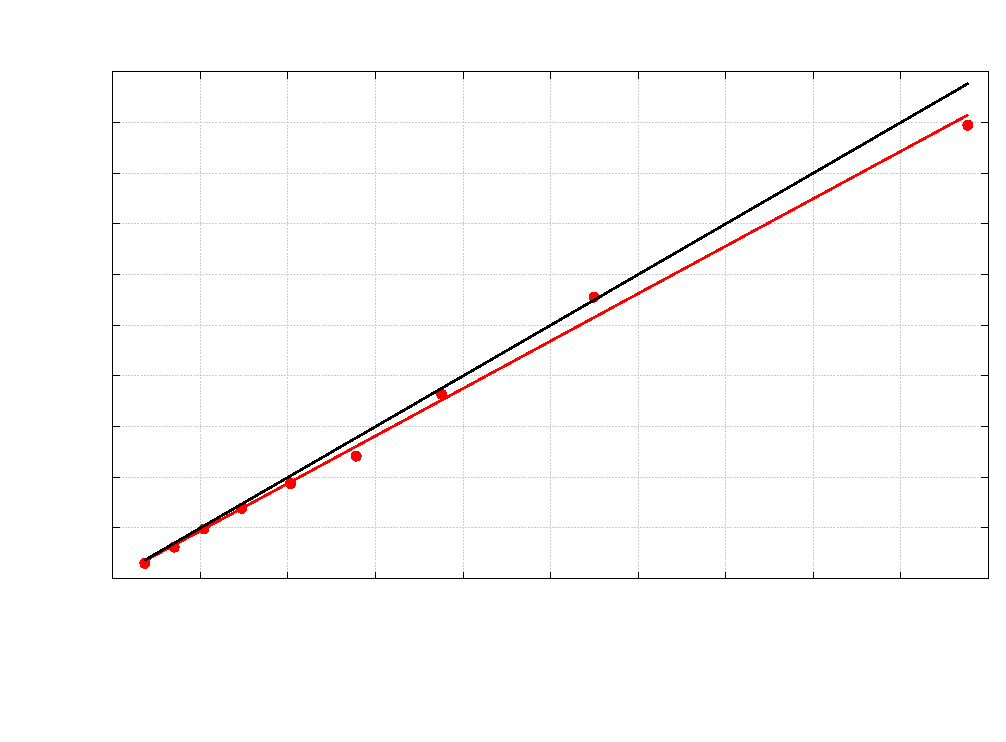
\includegraphics{plot3}}%
    \gplfronttext
  \end{picture}%
\endgroup
}
\end{center}
\end {figure}

\section*{RLC-резонанс}

Комплексный импеданс RLC-цепочки:
$$Z=R+j\omega L - \frac{j}{\omega C}.$$

Сдвиг фаз между током и напряжением получим, взяв аругмент $Z$:

$$\tg\varphi = \frac{\omega L - \frac{1}{\omega C}}{R} = Q\frac{\left(\frac{\omega}{\omega_0}\right)^2 - 1}{\frac{\omega}{\omega_0}} = Q\frac{(1+x)^2-1}{1+x} \simeq 2x Q,$$
где $x = \Delta \omega / \omega_0 = \Delta \nu / \nu_0$, и в последнем переходе пренебрегаем квадратичными по $x$ членами.
Измерив ширину графика $w=2x$ на высоте $\varphi = \pi / 4\ (\tg\varphi = 1)$, можем непосредственно измерить добротность контура:
$$Q = \frac{1}{w}$$

\begin {figure}[H]
\begin{center}
{% GNUPLOT: LaTeX picture with Postscript
\begingroup
  \fontfamily{sansserif}%
  \selectfont
  \makeatletter
  \providecommand\color[2][]{%
    \GenericError{(gnuplot) \space\space\space\@spaces}{%
      Package color not loaded in conjunction with
      terminal option `colourtext'%
    }{See the gnuplot documentation for explanation.%
    }{Either use 'blacktext' in gnuplot or load the package
      color.sty in LaTeX.}%
    \renewcommand\color[2][]{}%
  }%
  \providecommand\includegraphics[2][]{%
    \GenericError{(gnuplot) \space\space\space\@spaces}{%
      Package graphicx or graphics not loaded%
    }{See the gnuplot documentation for explanation.%
    }{The gnuplot epslatex terminal needs graphicx.sty or graphics.sty.}%
    \renewcommand\includegraphics[2][]{}%
  }%
  \providecommand\rotatebox[2]{#2}%
  \@ifundefined{ifGPcolor}{%
    \newif\ifGPcolor
    \GPcolorfalse
  }{}%
  \@ifundefined{ifGPblacktext}{%
    \newif\ifGPblacktext
    \GPblacktexttrue
  }{}%
  % define a \g@addto@macro without @ in the name:
  \let\gplgaddtomacro\g@addto@macro
  % define empty templates for all commands taking text:
  \gdef\gplbacktext{}%
  \gdef\gplfronttext{}%
  \makeatother
  \ifGPblacktext
    % no textcolor at all
    \def\colorrgb#1{}%
    \def\colorgray#1{}%
  \else
    % gray or color?
    \ifGPcolor
      \def\colorrgb#1{\color[rgb]{#1}}%
      \def\colorgray#1{\color[gray]{#1}}%
      \expandafter\def\csname LTw\endcsname{\color{white}}%
      \expandafter\def\csname LTb\endcsname{\color{black}}%
      \expandafter\def\csname LTa\endcsname{\color{black}}%
      \expandafter\def\csname LT0\endcsname{\color[rgb]{1,0,0}}%
      \expandafter\def\csname LT1\endcsname{\color[rgb]{0,1,0}}%
      \expandafter\def\csname LT2\endcsname{\color[rgb]{0,0,1}}%
      \expandafter\def\csname LT3\endcsname{\color[rgb]{1,0,1}}%
      \expandafter\def\csname LT4\endcsname{\color[rgb]{0,1,1}}%
      \expandafter\def\csname LT5\endcsname{\color[rgb]{1,1,0}}%
      \expandafter\def\csname LT6\endcsname{\color[rgb]{0,0,0}}%
      \expandafter\def\csname LT7\endcsname{\color[rgb]{1,0.3,0}}%
      \expandafter\def\csname LT8\endcsname{\color[rgb]{0.5,0.5,0.5}}%
    \else
      % gray
      \def\colorrgb#1{\color{black}}%
      \def\colorgray#1{\color[gray]{#1}}%
      \expandafter\def\csname LTw\endcsname{\color{white}}%
      \expandafter\def\csname LTb\endcsname{\color{black}}%
      \expandafter\def\csname LTa\endcsname{\color{black}}%
      \expandafter\def\csname LT0\endcsname{\color{black}}%
      \expandafter\def\csname LT1\endcsname{\color{black}}%
      \expandafter\def\csname LT2\endcsname{\color{black}}%
      \expandafter\def\csname LT3\endcsname{\color{black}}%
      \expandafter\def\csname LT4\endcsname{\color{black}}%
      \expandafter\def\csname LT5\endcsname{\color{black}}%
      \expandafter\def\csname LT6\endcsname{\color{black}}%
      \expandafter\def\csname LT7\endcsname{\color{black}}%
      \expandafter\def\csname LT8\endcsname{\color{black}}%
    \fi
  \fi
    \setlength{\unitlength}{0.0500bp}%
    \ifx\gptboxheight\undefined%
      \newlength{\gptboxheight}%
      \newlength{\gptboxwidth}%
      \newsavebox{\gptboxtext}%
    \fi%
    \setlength{\fboxrule}{0.5pt}%
    \setlength{\fboxsep}{1pt}%
\begin{picture}(9354.00,6802.00)%
    \gplgaddtomacro\gplbacktext{%
      \csname LTb\endcsname%
      \put(660,1669){\makebox(0,0)[r]{\strut{}$-\frac{\pi}{4}$}}%
      \csname LTb\endcsname%
      \put(660,2755){\makebox(0,0)[r]{\strut{}$-\frac{\pi}{8}$}}%
      \csname LTb\endcsname%
      \put(660,3841){\makebox(0,0)[r]{\strut{}$0$}}%
      \csname LTb\endcsname%
      \put(660,4926){\makebox(0,0)[r]{\strut{}$\frac{\pi}{8}$}}%
      \csname LTb\endcsname%
      \put(660,6012){\makebox(0,0)[r]{\strut{}$\frac{\pi}{4}$}}%
      \csname LTb\endcsname%
      \put(1391,968){\makebox(0,0){\strut{}$0.92$}}%
      \csname LTb\endcsname%
      \put(2324,968){\makebox(0,0){\strut{}$0.94$}}%
      \csname LTb\endcsname%
      \put(3258,968){\makebox(0,0){\strut{}$0.96$}}%
      \csname LTb\endcsname%
      \put(4191,968){\makebox(0,0){\strut{}$0.98$}}%
      \csname LTb\endcsname%
      \put(5125,968){\makebox(0,0){\strut{}$1$}}%
      \csname LTb\endcsname%
      \put(6059,968){\makebox(0,0){\strut{}$1.02$}}%
      \csname LTb\endcsname%
      \put(6992,968){\makebox(0,0){\strut{}$1.04$}}%
      \csname LTb\endcsname%
      \put(7926,968){\makebox(0,0){\strut{}$1.06$}}%
      \csname LTb\endcsname%
      \put(8859,968){\makebox(0,0){\strut{}$1.08$}}%
    }%
    \gplgaddtomacro\gplfronttext{%
      \csname LTb\endcsname%
      \put(-273,3840){\rotatebox{-270}{\makebox(0,0){\strut{}$\varphi$, рад}}}%
      \put(5125,308){\makebox(0,0){\strut{}$\nu / \nu_0$}}%
    }%
    \gplbacktext
    \put(0,0){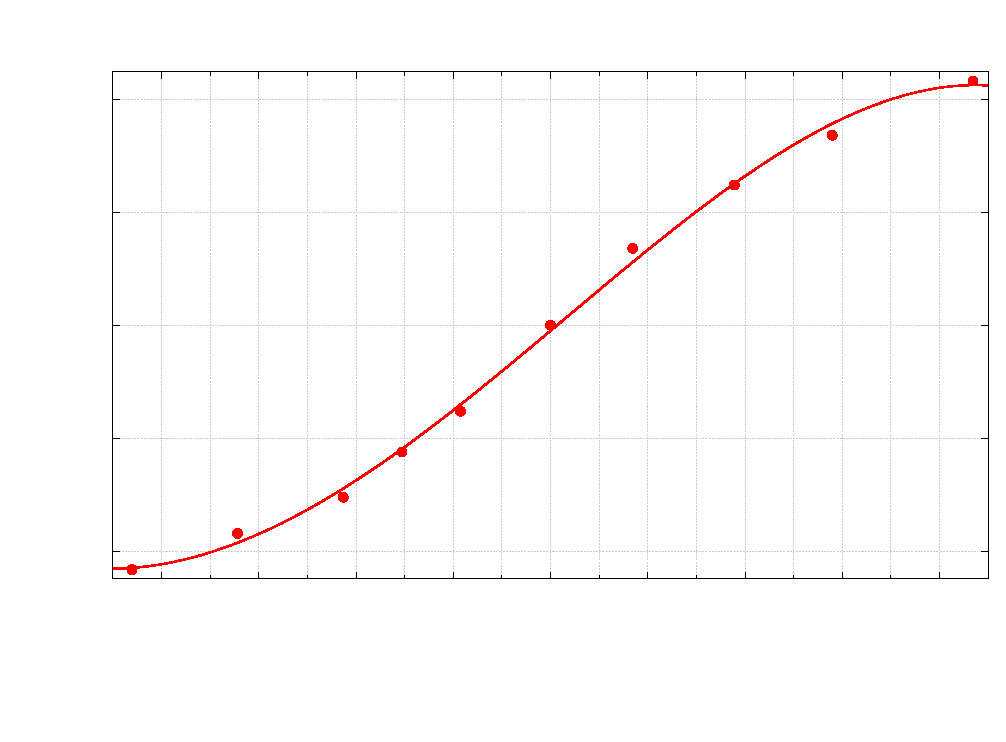
\includegraphics{rlc}}%
    \gplfronttext
  \end{picture}%
\endgroup
}
\end{center}
\end {figure}



Из графика добротность равна:
$$Q=7\pm1$$.

Можно рассчитать её, выразив через параметры цепочки:
$$Q = \frac{1}{R} \sqrt{\frac{L}{C}}$$
$$Q_{\text{теор}} = 5,7$$

\section*{Фазовращатель}

\begin {figure}[H]
\begin{center}
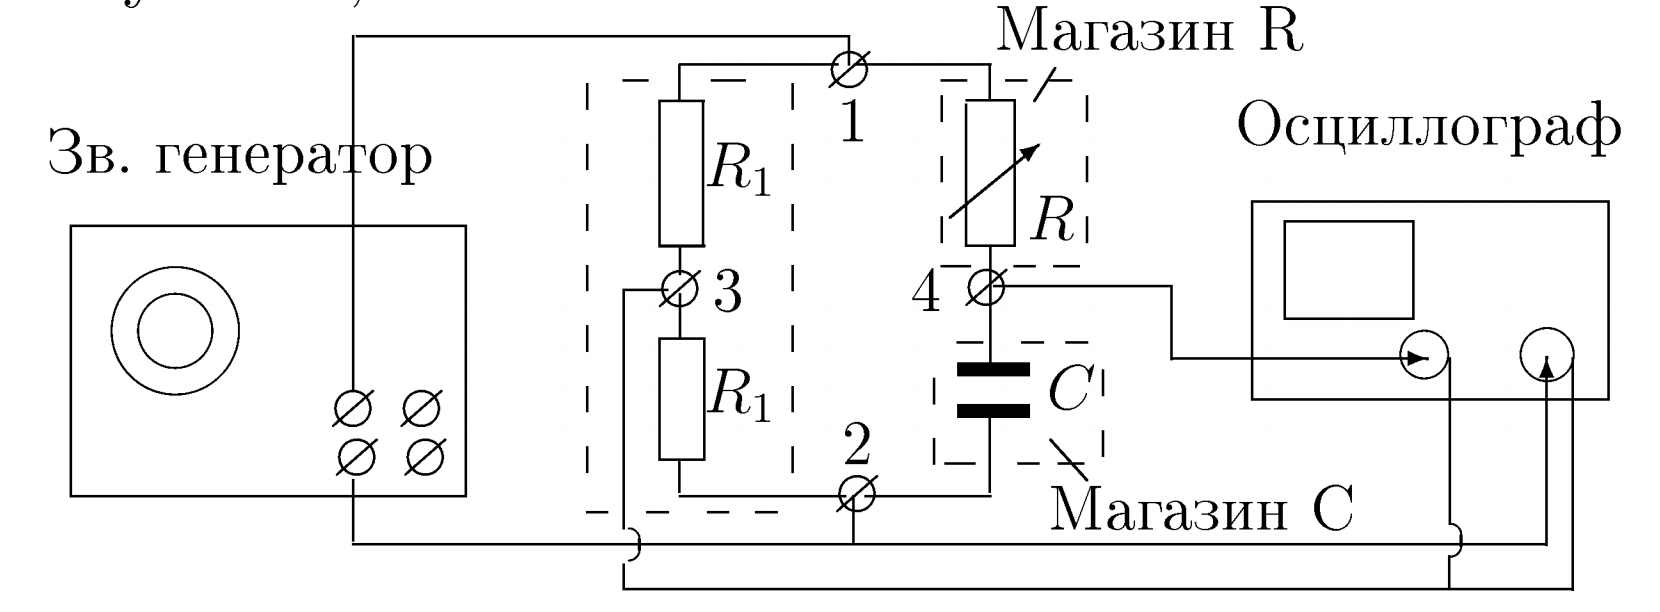
\includegraphics[width=0.8\textwidth]{phase.png}
\end{center}
\end {figure}


\begin {figure}[H]
\begin{center}
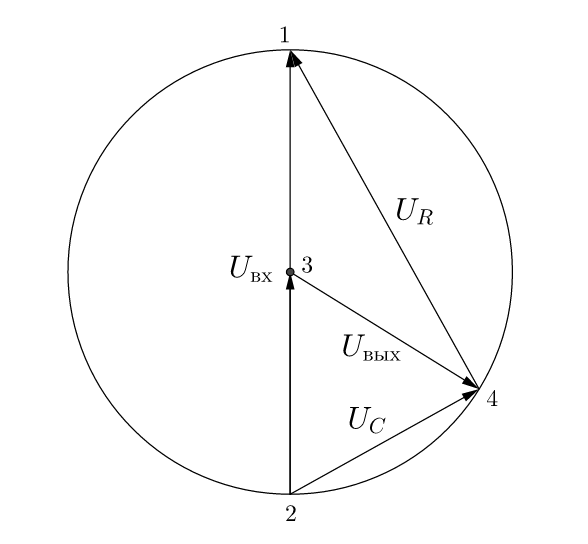
\includegraphics[width=0.7\textwidth]{diagramphase}
\end{center}
\end {figure}

Разность фаз равна $\pi /2$, когда медиана $34$ является и высотой, т.е. когда $\triangle 124$ -- равнобедренный, откуда

$$U_R=U_C,$$
$$R=\frac{1}{\omega C} = 318 \text{ Ом}$$
Измеренное на практике значение:
$$R_{\text{эксп}} = 336 \pm 25 \text{ Ом}$$ 
\end{document}